\documentclass[tikz,border=5pt]{standalone}
\usepackage[UTF8]{ctex}\usepackage{amsmath,amssymb}
\usetikzlibrary{arrows.meta,calc}
\definecolor{ink}{HTML}{243447}\definecolor{blue}{HTML}{2765A2}
\definecolor{green}{HTML}{3F7D5B}\definecolor{red}{HTML}{B74739}
\tikzset{body/.style={draw=ink,thick},vec/.style={draw=blue,thick,-{Latex}},guide/.style={gray!65,dashed},line cap=round,line join=round}
\begin{document}
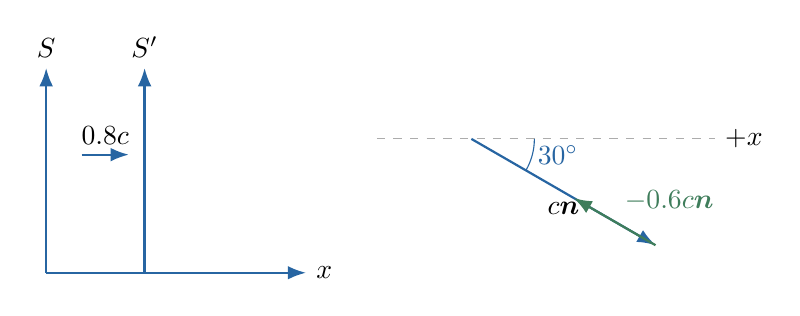
\begin{tikzpicture}
 \draw[vec](0,0)--(3.3,0)node[right]{$x$};\draw[vec](0,0)--(0,2.6)node[above]{$S$};
 \draw[vec](1.25,0)--(1.25,2.6)node[above]{$S'$};
 \draw[vec](.45,1.5)--(1.05,1.5)node[midway,above]{$0.8c$};
 \begin{scope}[xshift=5.4cm,yshift=1.7cm]
  \draw[guide](-1.2,0)--(3.1,0);\node[right]at(3.1,0){$+x$};
  \draw[vec](0,0)--({2.7*cos(30)},{-2.7*sin(30)})node[midway,below]{$c\boldsymbol n$};
  \draw[green,thick,-{Latex}]({2.7*cos(30)},{-2.7*sin(30)})--({1.5*cos(30)},{-1.5*sin(30)})node[midway,above right]{$-0.6c\boldsymbol n$};
  \draw[blue](.8,0)arc[start angle=0,end angle=-30,radius=.8];\node[blue]at(1.1,-.2){$30^\circ$};
 \end{scope}
\end{tikzpicture}
% 门平面的两个击中位置；入射与反射严格重走各自直线。
\begin{tikzpicture}
 \coordinate(E0)at(0,0);\coordinate(E1)at(1.333333,0);
 \coordinate(H0)at(3.247595,-1.875);\coordinate(H1)at(3.41465,-1.201656);
 \draw[vec](-.5,0)--(5.3,0)node[right]{$x$};
 \draw[blue,thick](E0)--(H0);\draw[red,thick](E1)--(H1);
 \draw[vec]($(E0)!.22!(H0)$)--($(E0)!.45!(H0)$);
 \draw[red,thick,-{Latex}]($(H0)!.28!(E0)$)--($(H0)!.5!(E0)$);
 \draw[red,thick,-{Latex}]($(E1)!.2!(H1)$)--($(E1)!.45!(H1)$);
 \draw[green,thick,-{Latex}]($(H1)!.2!(E1)$)--($(H1)!.45!(E1)$);
 \draw[green!55,dashed,thick]($(H0)+(-1,-1.73205)$)--($(H0)+(1,1.73205)$);
 \draw[green,thick]($(H1)+(-1,-1.73205)$)--($(H1)+(1,1.73205)$);
 \node[green,above right]at($(H1)+(1,1.73205)$){后一次门位置};
 \node[green!70!black,below right]at($(H0)+(1,1.73205)$){前一次};
 \foreach\p in{E0,E1,H0,H1}{\fill[ink](\p)circle(2pt);}
 \node[above left]at(E0){$E_0=R_0$};\node[above right]at(E1){$E_1=R_1$};
 \node[below left]at(H0){$H_0$};\node[above left]at(H1){$H_1$};
 \draw[green,thick,-{Latex}](5,-2.3)--(4.1,-1.78)node[midway,right]{门速度};
 \node at(2.5,-4){箭头表示不同传播方向，返回线与去程线重合};
\end{tikzpicture}
% x-ct投影：非完整三维时空图，不将投影斜率当光速。
\begin{tikzpicture}[x=1.25cm,y=.7cm]
 \draw[vec](-.15,0)--(4.6,0)node[right]{$x/(c\,\mathrm s)$};
 \draw[vec](0,-.2)--(0,8.5)node[above]{$t/\mathrm s$};
 \draw[guide](0,0)--(2.24,2.8);\node[gray]at(.9,2.5){$x=0.8ct$};
 \draw[blue,thick](0,0)--(3.247595,3.75);
 \draw[blue,thick,dashed](3.247595,3.75)--(0,7.5);
 \draw[red,thick](1.333333,1.666667)--(3.41465,4.069979);
 \draw[red,thick,dashed](3.41465,4.069979)--(1.333333,6.473291);
 \foreach\x/\y in{0/0,1.333333/1.666667,3.247595/3.75,3.41465/4.069979,0/7.5,1.333333/6.473291}{\fill[ink](\x,\y)circle(2pt);}
 \node[below left]at(0,0){$E_0$};\node[below right]at(1.333333,1.666667){$E_1$};
 \node[below right]at(3.247595,3.65){$H_0$};\node[above right]at(3.6,4.3){$H_1$};
 \draw[guide](3.41465,4.069979)--(3.6,4.3);
 \node[left]at(0,7.5){$R_0:\ 7.5$};\node[right]at(1.333333,6.473291){$R_1:\ 6.47329$};
 \draw[guide](1.333333,0)--(1.333333,1.5);
 \node[below]at(1.333333,0){$4/3$};
 \node at(2.2,-1){$D/c=6\,\mathrm s$；光路的 $x$—$t$ 投影};
\end{tikzpicture}
\end{document}
